\documentclass[floatfix,nofootinbib,superscriptaddress,fleqn,preprint]{revtex4} 
%\documentclass[aps,epsfig,tightlines,fleqn]{revtex4}
\usepackage[utf]{kotex}
\usepackage[HWP]{dhucs-interword}
\usepackage[dvips]{color}
\usepackage{graphicx}
\usepackage{bm}
%\usepackage{fancyhdr}
%\usepackage{dcolumn}
\usepackage{defcolor}
\usepackage{amsmath}
\usepackage{amsfonts}
\usepackage{amssymb}
\usepackage{amscd}
\usepackage{amsthm}
\usepackage[utf8]{inputenc}
 \usepackage{setspace}
%\pagestyle{fancy}

\begin{document}

\title{\Large 2021년 1학기 물리학 I: Quiz 9}
\author{김현철\footnote{Office: 5S-436D (면담시간 매주
    화요일-16:00$\sim$20:00)}} 
\email{hchkim@inha.ac.kr}
\affiliation{Hadron Theory Group, Department of Physics,
Inha University, Incheon 22212, Republic of Korea }
\date{Spring semester, 2021}


\vspace{1.cm}
\begin{abstract}
\noindent \textbf{ {\color{red}주의}: \color{blue} 단 한 번의 부정행위도 절대
  용납하지 않습니다. 적발 시, 학점은 F를 받게 됨은 물론이고,
  징계위원회에 회부합니다. One strike out임을 명심하세요.}\\
\\
문제는 다음 쪽부터 나옵니다.  \\ \\
{\bf Date:} 2021년 3월 30일 (화) 13:55-14:45 
\\
{\bf 학번:} \hspace{4cm}
{\bf 이름:} 

\end{abstract}
\maketitle

\noindent {\bf 문제 1. (30pt)} 
그림~\ref{fig:2}에서처럼
$\theta=30.0^\circ$만큼 기울어져 있는 면 위에 질량이 12.0 kg인
나무토막이 놓여있다. 이 토막 아래에는 270. N의 힘을 받으면 2.00 cm
만큼 압축되는 용수철이 놓여있다. 이 토박을 가만히 놓으면, 비탈면으로
내려와서 용수철을 5.50 cm 압축시킨다.
\begin{figure}[ht]
  \centering
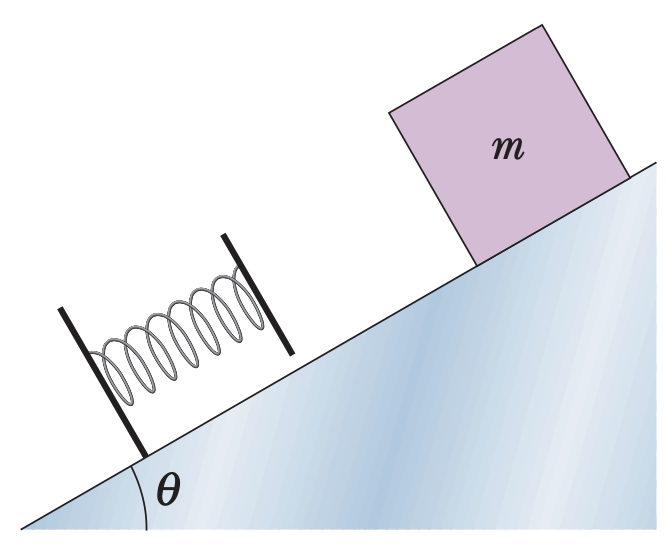
\includegraphics[scale=0.5]{Qfig9-2-20210330.png}  
  \caption{문제 2}
  \label{fig:2}
\end{figure}

\begin{itemize}
\item[(가)] 정지 상태에서 용수철을 압축시켜 멈추게 될 때까지 이
  나무토막은 얼마나 내려왔는가?
\item[(나)] 나무토막이 용수철에 닿는 순간의 속력은 얼마인가?   
\end{itemize}

\newpage
{\color{gray} [문제 풀이 쪽]}

\newpage

\noindent {\bf 문제 2. (50 pt)} 
어떤 아이가 그림~\ref{fig:2}처럼
반지름이 $R$인 반구 모양의 얼음 위에 앉아 있다가 무시할 수 있는 아주
작은 처음속력으로 미끄러지기 시작한다. 
\begin{figure}[ht]
  \centering
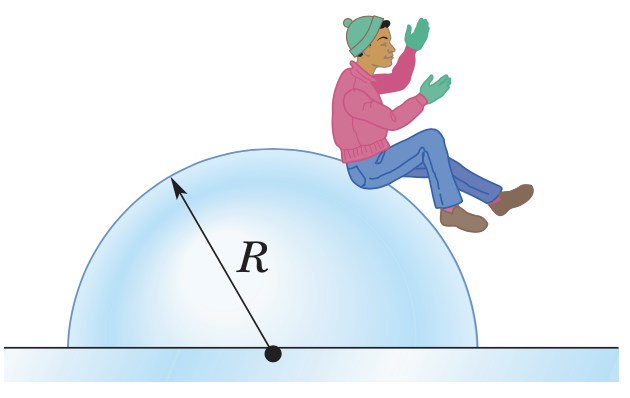
\includegraphics[scale=0.5]{Qfig9-3-20210330.png}  
  \caption{문제 2}
  \label{fig:2}
\end{figure}
얼음과 아이 사이에 쓸림이 없다고 가정한다면, 아이가 얼음에서 떠나는
높이는 어디인가?
  \newpage

{\color{gray} [문제 풀이 쪽]}

\newpage

\noindent {\bf 문제 3. (20 pt)}
그림~\ref{fig:3}의 암모니아 분자($\mathrm{NH}_3$)는 세 개의
수소원자(H)가 정삼각형의 꼭지점에 있고 정삼각형의 중심은
수소원자로부터 $d=9.40\times 10^{-11}$ m만큼 떨어져
있다. 질소원자(N)는 수소원자들이 바닥을 이루는 피라미드의 꼭지점에
있다. 질소 대 수소의 원자질량 비율은 13.9이고, 질소에서 수소까지의
거리는 $L=10.14\times 10^{-11}$ m이다. 
\begin{figure}[ht]
  \centering
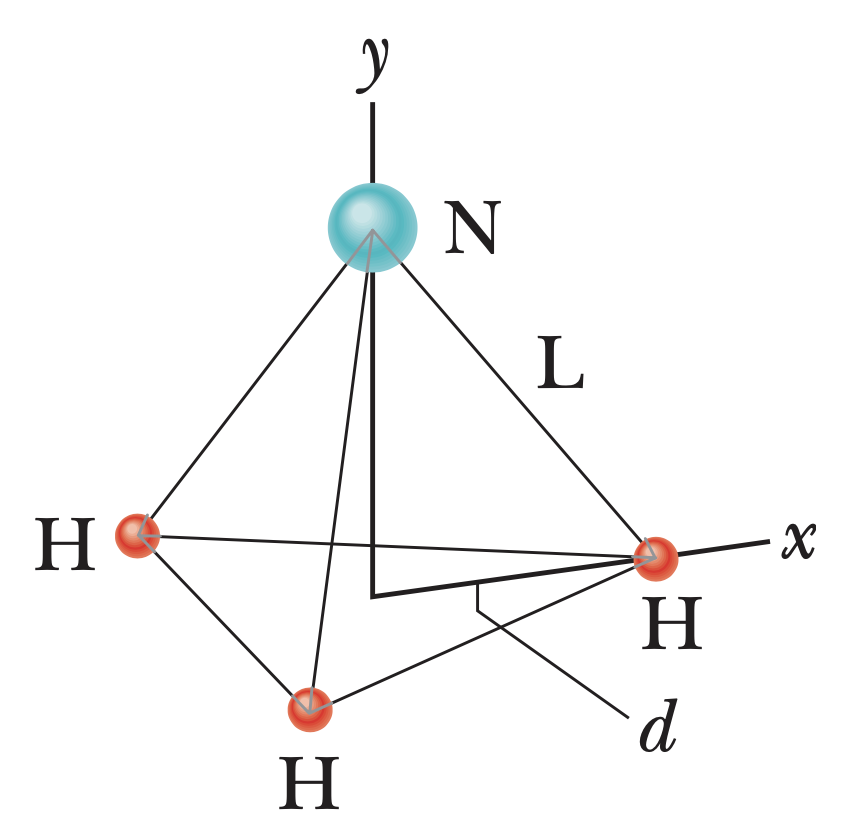
\includegraphics[scale=0.3]{Qfig9-4-20220330.png}  
  \caption{문제 3}
  \label{fig:3}
\end{figure}
암모니아분자의 질량중심의
\begin{itemize}
\item[(가)] $x$ 좌표
\item[(나)] $y$ 좌표는 각각 무엇인가? 
\end{itemize}
\newpage
{\color{gray} [문제 풀이 쪽]}

\newpage

\end{document}